\chapter{Sharing-aware data mapping in STM}\label{chap:sharAwareDataMap}

This appendix shows how STMap~(Section~\ref{sect:onlineThreadMapping}) can be extended to include sharing-aware \textbf{data mapping}. We opted for including the experiments on data mapping in the appendix since the main focus of this thesis is on sharing-aware \textbf{thread mapping}. The goal of data mapping is to optimize the usage of memory controllers, by mapping memory pages to the same NUMA node where the core that is accessing them belongs. To summarize, thread mapping aims to avoid access to the memory, prioritizing caches. On the other hand, if access to the memory is necessary, data mapping tries to map the memory that needs to be accessed to a local NUMA node, avoiding remote accesses.

\section{Algorithm}
To perform a sharing-aware data mapping in STM, it is necessary to know which NUMA nodes are accessing each memory page address. For this purpose, we follow the same intuition of the mechanism to detect thread communication, proposed in Section~\ref{sect:finalAlgorithmOnlineMap}, with some modifications, shown in \figurename~\ref{fig:mechanismDataMapping} and detailed in Algorithm~\ref{alg:commAndDataMap}.
\begin{figure}[!ht]
	%https://docs.google.com/presentation/d/1am8tJ-cKk_m5zLPlQp-dgm73BCcsaBYHSaLeyrmCFNo/edit?usp=sharing
	\centering
	\fbox{
		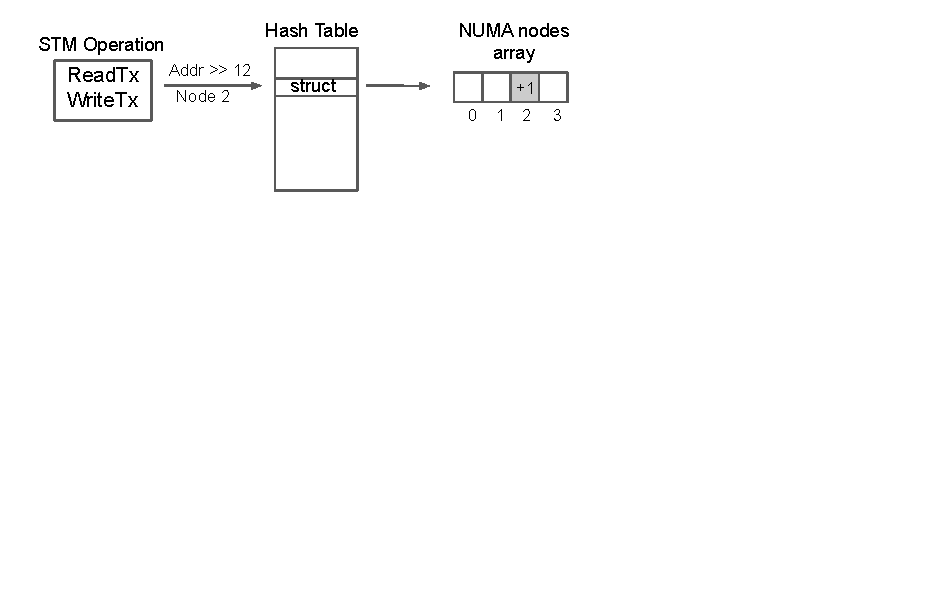
\includegraphics[width=0.8\textwidth,trim=10 170 160 0,clip]{figures/sharingAwareDataMapping/MechanismDataMapping.pdf}
	}
	\caption{Mechanism for detecting page accesses. Data structures are shown for a NUMA machine with 4 nodes (0-3).}
	\label{fig:mechanismDataMapping}
\end{figure}
\begin{algorithm}[ht]
	\caption{Detecting memory pages accesses and performing data mapping.}\label{alg:commAndDataMap}
	\begin{algorithmic}[1]
		\Require
		\Statex \textbf{addr}: memory address being accessed
		\Statex \textbf{node}: NUMA node that is accessing the memory page				
		%		\Statex tx: struct that contains data about the current transaction
		\Statex \textbf{tid}: thread ID of the thread that is accessing the address
		\Statex \textbf{addr\_sample} : thread private variable used to determine if is time to sample the memory address
		\Statex \textbf{total\_addr} : thread private variable used to determine if is time to trigger the thread mapping
		\Statex \textbf{si}: sample interval. Default 100
		\Statex \textbf{dmi}: data mapping interval. 
		\Statex \textbf{PAGE\_SIZE\_BITS}: 12 for page size of 4096 bytes
		\Statex
		%	\If {($collect\_comm$)} \label{alg2:shouldcollect}
		\State $addr\_sample \gets addr\_sample + 1$ \label{alg3:incsample}
		\If{($addr\_sample > si$)}  \label{alg3:samplegreater}
		\State $addr\_sample \gets 0$ \label{alg3:zerosample}
		\State $pageaddr \gets addr >> \text{PAGE\_SIZE\_BITS}$ \Comment{Right shift} \label{alg3:shiftaddr} 
		\State $elem \gets \text{getPageInfo}(pageaddr)$ \label{alg3:elem}
		\If {$(!elem.moved)$} \Comment{Verify if the memory page already have been moved} \label{alg3:moved}
		\State $elem.nodes[node]  \gets elem.nodes[node] +1$ \label{alg3:increaseAcc}	\Comment{Increase the amount of access}
		\EndIf
		\EndIf
		%			\LineComment{To avoid high overhead, for mapping purposes, only keep track of total address accessed by thread 1}
		\If {($tid = 1$)} \label{alg3:isthreadone}
		\State $total\_addr \gets total\_addr + 1$ \label{alg3:inctotaladdr}
		\EndIf
		\If {($tid = 1$)  \textbf{and} ($total\_addr \geq dmi$)} \label{alg3:istimetomap}
		\State Compute new data mapping \label{alg3:triggerdatamapping}
		\State $dmi \gets dmi * 2$ \label{alg3:increasedmi}
		\EndIf
		%		\EndIf
	\end{algorithmic}
\end{algorithm}

Lines \ref{alg3:incsample}, \ref{alg3:samplegreater} and \ref{alg3:zerosample} are exactly the same of the Algorithm~\ref{alg:commAndMap}~(Section~\ref{sect:finalAlgorithmOnlineMap}), i.e., it is used to verify if it is time to sample the accessed memory page, based on the value of sampling interval. Since the STM runtime has access to the full memory address, we first need to bit shift the address to get the information of the memory page (line \ref{alg3:shiftaddr}). To keep track of accessed memory pages, a hash table is used whose keys are memory pages. Each position of the hash table contains a structure with the memory address and an array of size equals to the NUMA nodes of the machine~(\figurename~\ref{fig:mechanismDataMapping}). Each position of this array contains the number of accesses to the memory page performed by each NUMA node. Hence,  on line \ref{alg3:elem}, the function \texttt{getPageInfo} gets from the hash table the structure containing information about the memory page being accessed. To avoid unnecessary page moves, we only update the number of accesses to this page (line \ref{alg3:increaseAcc}) if the page not already have been moved (line \ref{alg3:moved}). In summary, instead of calling Algorithm~\ref{alg:detectcomm}~(Chapter~\ref{chap:mechanism}) to detect the sharing behavior between threads, the modified algorithm keep track of the number of times which each NUMA node is accessing a specific memory page (lines \ref{alg3:shiftaddr}--\ref{alg3:increaseAcc}).

The lines \ref{alg3:isthreadone} to \ref{alg3:istimetomap} are the same of the Algorithm~\ref{alg:commAndMap}~(Section~\ref{sect:finalAlgorithmOnlineMap}), keeping track of the amount of memory address accessed, in order to trigger the data mapping. On the line \ref{alg3:triggerdatamapping} the data mapping is triggered. This step is simpler than thread mapping: we verify on the hash table each memory page that not have been moved and which NUMA node has most accessed it. Then, while the application is running, we send these information to the function \texttt{move\_pages} of the \texttt{libnuma} library~\cite{libnuma} to perform the page move.

Contrary to thread mapping, where our previous study showed that \texttt{STAMP} applications do not present dynamic sharing behavior (Chapter~\ref{chap:charact}), hence, not being necessary to perform more than one time the thread mapping, on data mapping we cannot disable the mechanism after the first trigger. For thread mapping, just keeping track of a few memory accesses it is possible to deduce, with a certain level of accuracy, the memory access pattern of the application. For data mapping, it is not possible to deduce the future memory pages that will be accessed and which NUMA nodes will access them. However, to avoid a high overhead of moving pages, after each data mapping, on line \ref{alg3:increasedmi}, we double the next \emph{data mapping interval} (dmi). 

\section{Improving STM applications with Data Mapping}\label{sect:dataMappingProof}
%In order to verify if the proposed mechanism to explore data mapping inside STM runtime work correctly

Similar to the experiment made on Section~\ref{sec:improvements} for thread mapping, we create an experiment with a synthetic array sum application. This application consists of an array of $2^{30}$ integer elements. In that case, the array uses approximately 4 Gigabytes of memory. We force the array to be initialized with zeros in the main thread. Hence, using the default \emph{first touch} police, all memory will be allocated in the NUMA node of the main thread. To force the use of more than one NUMA node, the application was executed using 64 threads. The objective of this application is very simple. Each thread iterates through their array part thirty times. On each iteration, it updates the respective array position, incrementing the current value by one. We implemented the proposed mechanism of this Appendix inside the \texttt{TinySTM} and used it for synchronization of shared variables used in the array. 
%We use the proposed mechanism in this appendix to protect the modification of each array position. 
Hence, the STM runtime will be aware of all the memory addresses that belong to the array. We iterate through the array thirty times to guarantee that if a memory page is migrated then it will be accessed again in the appropriate NUMA node, regarding the locality of the access.

The default Linux kernel already has routines to improve the memory page balancing of NUMA nodes. It keeps track of the page faults, moving the page automatically to the node that most accessed it. This mechanism is called \emph{NUMA balancing}~\cite{NumaB:2020}. To test our proposal, we executed the array sum application in the Xeon and Opteron machines, described in Section~\ref{sect:threadMapMethodology}. For comparison we used the following configurations:

\begin{itemize}
	\item \textbf{Linux-NBOff} is the default Linux CFS scheduler, however with the NUMA balancing mechanism disabled.
	
	\item \textbf{Linux-NBOn} is the default Linux CFS scheduler with the NUMA balancing mechanism enabled. This approach will be useful to verify if the application is suitable for data mapping, or if the default \emph{first-touch} approach is more efficient.
	
	\item \textbf{STMap} is the mechanism proposed in Section.~\ref{sect:onlineThreadMapping}. However, since we are interested in verifying the benefits of data mapping together with thread mapping, we do not use the heuristic proposed in Algorithm~\ref{alg:enableMappig}, hence, the thread mapping is always triggered one time. 
	
	\item \textbf{STMap+DM} in this approach, we first trigger the thread mapping one time. After that, we begin to keeping track of the memory pages being accessed, triggering the first data mapping on \emph{dmi} of 100,000 addresses such as in thread mapping (Sect~\ref{sect:onlineThreadMapping}). 
\end{itemize}

\begin{figure}[!ht]
	\centering
	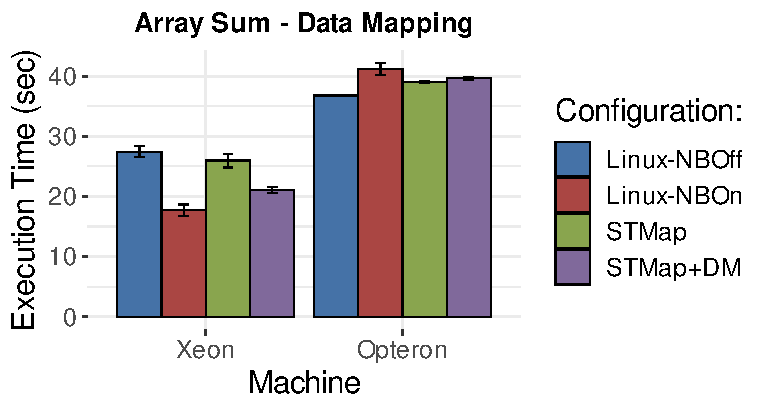
\includegraphics[width=0.7\textwidth]{figures/sharingAwareDataMapping/ArraySumDataMapping.pdf}
	\caption{Execution time of the Array Sum application.}
	\label{fig:arraySumDataMapping}
\end{figure}

It is worth noting that the \emph{NUMA balancing}~\cite{NumaB:2020} was enabled only in \textbf{Linux-NBOn} approach. In all other approaches, this mechanism was disabled. \figurename~\ref{fig:arraySumDataMapping} show the results. In the Xeon machine, it is possible to observe that NUMA balancing (\textbf{Linux-NBOn}) reduced the execution time by 35.5\% when compared to the same mechanism without the balancing (\textbf{Linux-NBOff}). This proves that this synthetic application has an unbalanced memory page allocation. Although it was not possible to beat NUMA balancing, our proposed \textbf{STMap+DM} mechanism achieved performance gains of 23.3\% when compared to \textbf{Linux-NBOff} and, 19\% when compared to \textbf{STMap}. However, when analyzing the results in the Opteron machine, it is not possible to see any benefits of the data mapping. In fact, NUMA balancing decreases the performance by 12\% when compared to \textbf{Linux-NBOff}. %Our STMap+DM mechanism decreased the performance by 7.8\%.

As related in Section~\ref{sect:threadMapMethodology} the information about NUMA nodes distances gathered with \texttt{numactl}~\cite{libnuma} indicates that the nodes distances in the Xeon machine are three times more distant than Opteron. This could explain in part the lack of results for data mapping in Opteron. To be sure about this information, we used a tool\footnote{\url{https://github.com/matthiasdiener/numafac}} to calculate the NUMA factor of the two machines, regarding bandwidth and latency of remote accesses. This tool uses \texttt{Lmbench}~\cite{lmbench} to calculate the latencies. The NUMA factor is defined as the latency between memory accesses to remote NUMA nodes divided by the latency to access local nodes~\cite{Mariano:2016}. \tablename~\ref{tab:NodeDistances} show the results. 
\begin{table}[h!tb]
	\centering
	\caption{NUMA factor of the machines used in the experiments.}
	\label{tab:NodeDistances}
	\begin{tabular}{@{}lcll@{}}
		\toprule
		&                         & \multicolumn{2}{c}{\textbf{NUMA factor}} \\ \cmidrule{3-4}
		\textbf{Machine} & \textbf{Node distances} & \textbf{Bandwidth}   & \textbf{Latency}  \\ \midrule
		Xeon             & 50 -- 65                & 1.96                 & 6.90              \\
		Opteron          & 16 -- 22                & 1.28                 & 2.16              \\ \bottomrule
	\end{tabular}
\end{table}
Although the bandwidth of the Xeon machine is larger than Opteron, the latency of remote accesses is three times slower in Xeon. This could explain in part why the array sum application only presented results on the Xeon machine. Nevertheless, in Section~\ref{sect:resultsDataMapping} we will test the proposed data mapping mechanism using more realistic workloads.


\section{Methodology}

Although the experiments made on Section~\ref{sect:dataMappingProof} with the array sum application were not conclusive regarding the Opteron machine, we executed all eight benchmarks from \texttt{STAMP} and the two micro-benchmarks (HashMap and Redblacktree) using the proposed data mapping mechanism. The \texttt{STAMP} applications represent realistic workloads, being more appropriate to verify the efficiency of the proposed mechanism. We also added two more mechanisms to the comparison:

\begin{itemize}
	\item \textbf{DM-100K} in this approach the thread mapping is not used, only data mapping, triggering the first mapping on 100,000 addresses. 
	
	\item \textbf{DM-50K} this approach is used to verify if a more aggressive data mapping is better, triggering the first mapping on 50,000 addresses, i.e., half of the previous approach.
\end{itemize}


\section{Results}\label{sect:resultsDataMapping}
%/home/douglas/GitRepo/ThesisFiles/04.DataMapping/ThreadDataMap/Xeon
%/home/douglas/GitRepo/ThesisFiles/04.DataMapping/JustDataMap/Opteron

The results of sharing-aware data mapping in both machines were similar. Hence, we will not discuss each application individually. Alternatively, we calculated the average speedup %(by using the geometric mean) 
using \textbf{Linux-NBOff} as a baseline. Also, the results were grouped by thread number and machine. \figurename~\ref{fig:ResultsSpeedupDataMap} show the results.

\begin{figure}[ht]
	\centering
	\subfigure[Xeon]{
		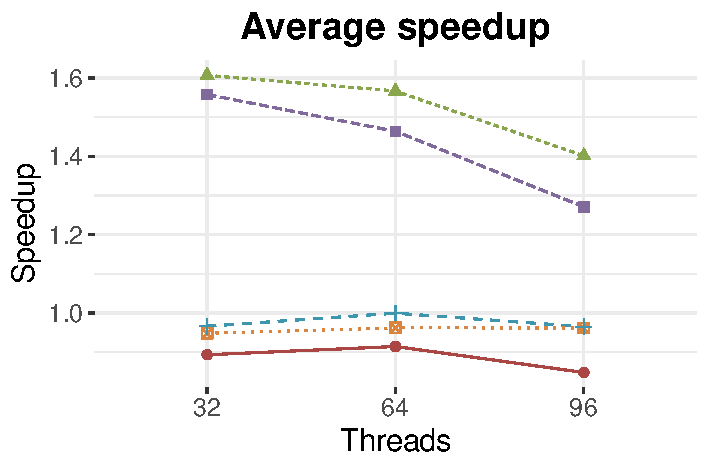
\includegraphics[width=\halfPage\textwidth]{figures/sharingAwareDataMapping/average_Speedup_xeon.pdf}
	}%
	\subfigure[Opteron]{
		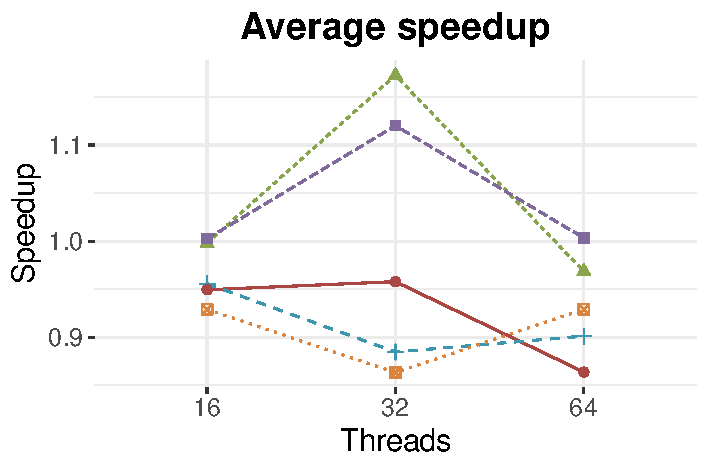
\includegraphics[width=\halfPage\textwidth]{figures/sharingAwareDataMapping/average_Speedup_opteron.pdf}
	}\\
	\subfigure{
		
\includegraphics[width=0.9\textwidth]{figures/sharingAwareDataMapping/legend_speedup.pdf}
	}%
	\caption{Average speedup of the mappings when compared to Linux-NOff.}
	\label{fig:ResultsSpeedupDataMap}
\end{figure}

Overall, the proposed mechanism does not improve the performance of STM applications. The best speedup was achieved by STMap, i.e., only triggering thread mapping, with exception of Opteron in 64 threads. When the data mapping was enabled together with thread mapping (\textbf{STMap+DM}) it decreased the performance. In that case, the overhead of the data mapping mechanism was not compensated by the better exploration of the locality of memory pages. However, analyzing the speedup, overall, on both machines the NUMA balancing mechanism (\textbf{Linux-NBOn}) decreased the performance. On the Xeon machine, all proposed mechanisms performed better than NUMA Balancing. In that case, the default \emph{first-touch} police were more efficient. Hence, initially, two hypotheses can be formulated. The first is that the applications utilized in the experiments are not suitable for data mapping. The second is that the proposed mechanism failed in exploring data mapping. However, this second hypothesis was tested in Sect~\ref{sect:dataMappingProof} and showed results in the Xeon Machine.

\section{Discussion}\label{sect:DataMappingDiscussion}

Albeit the proposed mechanism in this appendix does not improve the performance of the STM applications used in the previous chapters, a synthetic application showed that in specific scenarios it can improve the performance. More specifically, it is necessary an STM application with atomic blocks that protect a large amount of distinct variables and a NUMA machine with high latency in remote node accesses.

Since STM runtime has precise information about shared variables, this information can be used to choose which threads should be mapped closer to each other to share caches, i.e., it is not necessary a global vision of the application sharing behavior (Chapter~\ref{chap:sharAwareThreadMap}). However, for an efficient data mapping, it is necessary a global vision of the memory pages of the application, not only the ones accessed by the STM runtime. In the synthetic array sum application presented in Sect~\ref{sect:dataMappingProof}, the STM runtime was aware of all the 4 Gigabytes of the array. Nevertheless, data mapping showed improvements only in the Xeon machine, with high latencies on remote node access.

Using more realistic workloads, we do not see performance improvements. Probably, in the majority of STM applications, the STM runtime is not aware of the entire memory pages of the application. 


\section{Summary}
This appendix proposed an extension to STMap to include sharing-aware data mapping. The extension keeps track of the number of accesses of each NUMA node to each memory page. On each data mapping interval, the memory page is moved to the NUMA node that most accessed it. 

Using a synthetic array sum application, it was showed that the proposed mechanism could increase the performance on NUMA machines with high latency on remote memory access. However, using more realistic workloads, it was not possible to improve the performance. Our thoughts are that it could be infeasible to perform a sharing-aware data mapping take into consideration only STM operations because it represents only a fraction of the memory pages used by the entire application.
